\begin{frame}
  \frametitle{L�gicas modales}
  \begin{center} $ p \equiv "$Hoy hace fr�o$"$ \end{center}
  \visible<2->{
    \begin{itemize}
    \item �Hace realmente fr�o?
    \item �Es sabido que hoy hace fr�o?
    \item �Hace fr�o ahora, o dentro de un rato?
    \item Si vuelo a Dubl�n, �seguir� haciendo fr�o?
    \end{itemize}
  }
\end{frame}

%===================================
\sectionDark{L�gica epist�mica} %===
% ===================================
\begin{frame}
  \frametitle{L�gica epist�mica (1 agente)}
  \vspace{0.8cm}
  \begin{columns}
    \begin{column}{0.5\textwidth}
      L�gica proposicional:
      \begin{itemize}
      \item $p, q, \cdots \in \mathcal{P}$
      \item $\varphi,\quad \neg\varphi,\quad \varphi\mor\psi,\quad \varphi\mand\psi$
      \item $\varphi \rightarrow \psi $ ( $\myeq \neg\varphi \mor \psi$ )
      \end{itemize}
    \end{column}
    \begin{column}{0.5\textwidth}
      \visible<2->{
        L�gica epist�mica:
        \begin{itemize}
        \item $\K\,\varphi$\hspace{2.5cm}
        \item $\M\,\varphi \myeq \neg\K\neg\varphi$\hspace{0.9cm}
        \end{itemize}
      }
    \end{column}
  \end{columns}
  \vspace{1cm}
  \visible<3->{
    \begin{align*}
      \K(\varphi \rightarrow \psi): & \hspace{0.3cm} \text{``Se sabe que }
                                      \varphi \text{ implica } \psi\text{'' }\\
      \K \varphi \mor \K \neg \varphi: & \hspace{0.3cm} \text{``Se sabe que }
                                         \varphi \text{ o }
                                         \neg\varphi\text{'' } \\
      \K \varphi \mor \neg \K \varphi:  &\hspace{0.3cm} \text{``Puede que se sepa
                                          o no que }\varphi \text{'' } \\
    \end{align*}
  }
\end{frame}


%%%%%%%%%%%%%%%%%%%%%%%
% Kripke's structures %
%%%%%%%%%%%%%%%%%%%%%%%
\begin{frame}
  \frametitle{Modelo de mundos posibles\footnote{Formalizaci�n: Estructuras
    de Kripke}}
  \begin{center}{ $ \MM =\,< W, R, V >$}\end{center}
  \vspace{0.1cm}
  \begin{tabular}{ll}
    $W = \{w_1, w_2, w_3, \ldots \}$& Conjunto de mundos (o estados)
                                      posibles. \\
    $ R \subseteq W \times W $ & Operador de relaci�n entre
                            mundos. \\
    $ V: \varphi \rightarrow W' \subseteq W $ & En qu� mundos es cierta una f�rmula. \\
  \end{tabular}
  

  \vspace{1cm}
  
  \begin{block}{Ejemplo:}
    \begin{columns}
      \begin{column}{0.3\textwidth}
        \vspace{0.2cm} 
        \mbox{$p = $ ``Hoy es viernes''}\\ 
        \mbox{$q = $ ``Hoy es s�bado''}
        \vspace{1.5cm}
      \end{column}
      \begin{column}{0.5\textwidth}
        \vspace{1.3cm}
        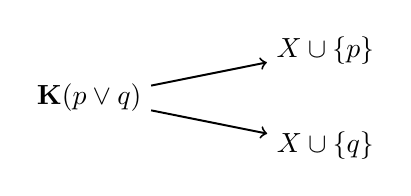
\begin{tikzpicture}[scale=1]
          \node [] (K) at (0.0, 0.6) {$\textbf{K} ( p \vee q ) $};
          \node [] (p) at (3, 1.2) {$X \cup \{p\}$};
          \node [] (q) at (3.0, 0.0) {$X \cup \{q\}$};
          
          \draw [line width = 0.25mm, ->] (K) -- (p);
          \draw [line width = 0.25mm, ->] (K) -- (q);
        \end{tikzpicture}
      \end{column}
    \end{columns}
  \end{block}
\end{frame}


%%%%%%%%%%%%%%%%%%%%%%%%%%%%%%%%
\sectionDarkSpecial{Ejemplo} %%%
%%%%%%%%%%%%%%%%%%%%%%%%%%%%%%%%
\begin{frame}
  \frametitle{Ejemplo}
  \begin{columns}
    \begin{column}{0.55\textwidth}
      Suponemos que existen \alert{tres cartas} (1, 2 y 3):\\
      -- Alicia tiene una carta en la mano.\\
      -- Otra est� bocabajo en la mesa.\\
      -- La �ltima se devuelve al mont�n.\\
      
      %-- Dynamic text
      \begin{overlayarea}{\textwidth}{4cm}
        \vspace{0.5cm}
        %-- Con numeros
        \only<2,3>{\textbf{�Cu�les son los estados relevantes?}\\}
        \only<4,5,6>{\textbf{�Qu� informaci�n tiene Alicia?}\\}
        \only<7,8>{
          $H_i \myeq $ ``Alicia tiene la carta $i$''\\
          $T_i \myeq $ ``La carta $i$ est� en la mesa''\\

          \begin{align*}
            \text{Ej.:} & V(H_1) = \{ w_1, w_2\}\\
                        & V(T_2) = \{ w_1, w_6 \} \\
          \end{align*}          
        }        
        %-- Con propiedades
        \only<9->{
          Supongamos que Alicia recibe la carta 1, y la carta 2 est� en la mesa.
        }
        \begin{itemize}[<+(9)->]
        \item[]
        \item[] $\MM, w_1 \models \K H_1$
        \item[] $\MM, w_1 \models \K \neg T_1$
        \item[] $\MM, w_1 \models \K (T_2 \mor T_3)$
        \end{itemize}
      \end{overlayarea}

    \end{column}
    \begin{column}{0.55\textwidth}
      % -- N�meros
      \only<3-7>{
        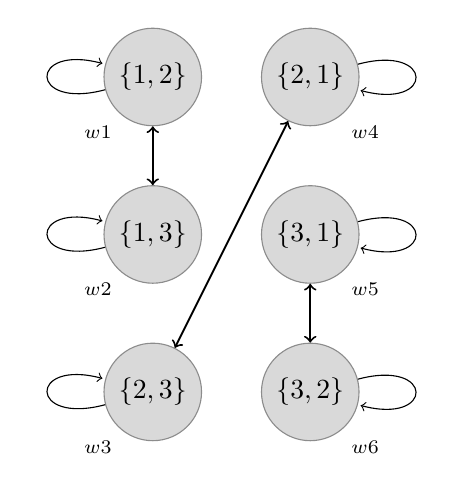
\begin{tikzpicture}[scale=1, transform shape]
          \tikzstyle{every node} = [circle, fill=gray!30, draw=gray!90] 
          \node [label=below left:\scriptsize$w1$] (w1) at (0.0, 4) {$\{1,2\}$};
          \node [label=below right:\scriptsize$w4$] (w4) at (2, 4) {$\{2,1\}$};
          \node [label=below left:\scriptsize$w2$] (w2) at (0.0, 2.0) {$\{1,3\}$};
          \node [label=below right:\scriptsize$w5$] (w5) at (2, 2.0) {$\{3,1\}$};
          \node [label=below left:\scriptsize$w3$] (w3) at (0.0, 0.0) {$\{2,3\}$};
          \node [label=below right:\scriptsize$w6$] (w6) at (2, 0.0) {$\{3,2\}$};
          \visible<5->{
            \draw [line width = 0.25mm, <->] (w1) -- (w2);
            \draw [line width = 0.25mm, <->] (w3) -- (w4);
            \draw [line width = 0.25mm, <->] (w5) -- (w6);
          }
          \visible<6->{
            \path [->] (w1) edge[loop left] ();
            \path [->] (w2) edge[loop left] ();
            \path [->] (w3) edge[loop left] ();
            \path [->] (w4) edge[loop right] ();
            \path [->] (w5) edge[loop right] ();
            \path [->] (w6) edge[loop right] ();
          }
        \end{tikzpicture}
      }
      % -- Prop

      \only<8->{
        \begin{tikzpicture}[scale=0.8, transform shape]
          \tikzstyle{every node} = [circle, fill=gray!30, draw=gray!90] 
          \only<-9>{\node [label=below left:\scriptsize$w1$] (w1) at (-0.2, 4.4) {$\{H_1,T_2\}$};}
          \only<10>{\node [label=below left:\scriptsize$w1$, line
            width=0.04cm, draw=black!100] (w1) at (-0.2, 4.4) {$\{H_1,T_2\}$};}
          \only<11->{\node [label=below left:\scriptsize$w1$, line
            width=0.04cm, draw=black!100, fill=blue!30] (w1) at (-0.2, 4.4) {$\{H_1,T_2\}$};}
          \node [label=below right:\scriptsize$w4$] (w4) at (2.2, 4.4) {$\{H_2,T_1\}$};
          \only<-10>{\node [label=below left:\scriptsize$w2$] (w2) at
            (-0.2, 2.0) {$\{H_1,T_3\}$};}
          \only<11->{\node [label=below left:\scriptsize$w2$, fill=blue!30] (w2) at (-0.2, 2.0) {$\{H_1,T_3\}$};}
          \node [label=below right:\scriptsize$w5$] (w5) at (2.2, 2.0) {$\{H_3,T_1\}$};
          \node [label=below left:\scriptsize$w3$] (w3) at (-0.2, -0.4) {$\{H_2,T_3\}$};
          \node [label=below right:\scriptsize$w6$] (w6) at (2.2, -0.4) {$\{H_3,T_2\}$};

          \only<-10>{\draw [line width = 0.25mm, <->] (w1) -- (w2);}
          \only<11->{\draw [line width = 0.25mm, <->, draw=blue!100] (w1) -- (w2);}
          \draw [line width = 0.25mm, <->] (w3) -- (w4);
          \draw [line width = 0.25mm, <->] (w5) -- (w6);
          
          \only<-10>{\path [->] (w1) edge[loop left] ();}
          \only<11->{\path [->, draw=blue!100] (w1) edge[loop left] ();}
          \path [->] (w2) edge[loop left] ();
          \path [->] (w3) edge[loop left] ();
          \path [->] (w4) edge[loop right] ();
          \path [->] (w5) edge[loop right] ();
          \path [->] (w6) edge[loop right] ();
        \end{tikzpicture}
      }
    \end{column}
  \end{columns}
\end{frame}



%%%%%%%%%%%
% Demostraciones
\sectionDark{Demostraciones (Tableaux)}
%%%%%%%%%%%

\begin{frame}
  \frametitle{Axiomas}
  
  \begin{table}
    \centering
    \begin{tabular}{lll} \toprule
      L�gica & Condici�n & Axioma \\ \midrule
      K & - & $\K ( \varphi \rightarrow \psi) \rightarrow (\K
                           \varphi \rightarrow \K \psi)$\\
      T & Reflexiva & $ \K\,\varphi \rightarrow \varphi $\\
      B & Reflexiva, sim�trica & $ \varphi \rightarrow \K\,\M\,\varphi$\\
      4 & Transitiva & $ \K \varphi \rightarrow \K\,\K\,\varphi$\\
      5 & Eucl�dea & $ \M \varphi \rightarrow \K\,\M\,\varphi$\\
      \bottomrule
    \end{tabular}
  \end{table}
  
  Seg�n que axiomas se acepten, se dan distintos tipos de sistemas:
  \begin{itemize}
  \item K4
  \item K5
  \item S4 = KT4
  \item S5 = KT5
  \end{itemize}
\end{frame}


\begin{frame}
  \frametitle{Reglas para tableaux epist�micos}
  \begin{table}
    \centering
    \begin{tabular}{lcccc} \toprule
      \vspace{0.4cm}Nombre & (K) & (T) & (S4) & (5) \\ 
      \vspace{0.2cm}Regla &       
              \AxiomC{$\K\,X;\neg\K\,\varphi$}
              \UnaryInfC{$X;\neg\varphi$}
              \DisplayProof
            &
              \AxiomC{$X;\K\,\varphi$}
              \UnaryInfC{$X;\{\K\,\varphi,\varphi\}$}
              \DisplayProof
            &
              \AxiomC{$\K\,X;\neg\K\,\varphi$}
              \UnaryInfC{$\K\,X;\neg\varphi$}
              \DisplayProof
            &
              \AxiomC{$X;\neg\K\,\varphi$}
              \UnaryInfC{$X;\neg\K\,\varphi;\K\neg\K\varphi$}
              \DisplayProof\\ \bottomrule
    \end{tabular}
  \end{table}

  \visible<2->{
    \begin{table}
      \centering
      \begin{tabular}{cccc} \toprule
        \vspace{0.4cm}Dualidad & Dualidad & Regla $\K$ & Regla $\M$  \\
        $\neg \K\,\varphi,\,i$ &$\neg\M\,\varphi,\,i$ & $\K\,\varphi,\,i$
                                                       &$\M\,\varphi,\,i$
        \\
        $\downarrow$ & $\downarrow$ & iRj & iRj \\
        $\M\neg\varphi,\,i$&
                             $\K\neg\varphi,\,i$&$\downarrow$&$\downarrow$\\
        &&$\varphi,\,j$&$\varphi,\,j$\\
                                                  
        \\ \bottomrule
      \end{tabular}
    \end{table}
  }

\end{frame}

%
%
%%%
%%% Local Variables:
%%% mode: latex
%%% TeX-master: "./carcasa.tex"
%%% End:
